\section{Wechsel- und Drehstromrechnung}
\begin{multicols}{3}
	\textbf{Ohmscher Widerstand $R$} \\
	$u$ und $i$ können sprunghaft ändern \\
	$u(t) = R \cdot i(t)$ \\
	$i(t) = \frac{u(t)}{R}$ \\
	$\underline{Z} = R$ \\ \\
	$\underline{Z} = R + jX = \lvert Z \rvert \cdot e^{j\varphi} = \frac{\underline{U}^2}{\underline{S}^*}$ \\
	$\underline{S} = \underline{U} \cdot \underline{I}^*$\\
	verkettete Spannung $U$: $U = \sqrt{3} \cdot U_{Str}$
	
	\textbf{Kapazität $C$} \\
	$u$ kann nicht sprunghaft ändern \\
	$u(t) = \frac{1}{C} \int_{0}^{t} i(\tau) d\tau + u(0)$ \\
	$i(t) = C\frac{du(t)}{dt}$ \\
	$\underline{Z} = \frac{1}{j \cdot \omega \cdot C} = -j \frac{1}{\omega \cdot C}$ \\ \\
	$\lvert \underline{Z} \rvert = Z = \frac{U}{I} = \sqrt{R^2 + X^2}$ \\
	$P = \Re(\underline{S}) = U \cdot I \cdot \sin \varphi$
	
	\textbf{Induktivität $L$} \\
	$i$ kann nicht sprunghaft ändern
	$u(t) = L\frac{di(t)}{dt}$ \\
	$i(t) = \frac{1}{L} \int_{0}^{t} u(\tau) d\tau + i(0)$ \\
	$\underline{Z} = j \cdot \omega \cdot L$ \\ \\
	$\varphi = \arctan \left(\frac{\Im (\underline{Z})}{\Re (\underline{Z})}\right) = \arctan \left(\frac{X}{R}\right)$ \\
	$Q = \Im (\underline{S}) = U \cdot I \cdot \sin \varphi$
\end{multicols}

\begin{minipage}[lt]{3.5cm}
	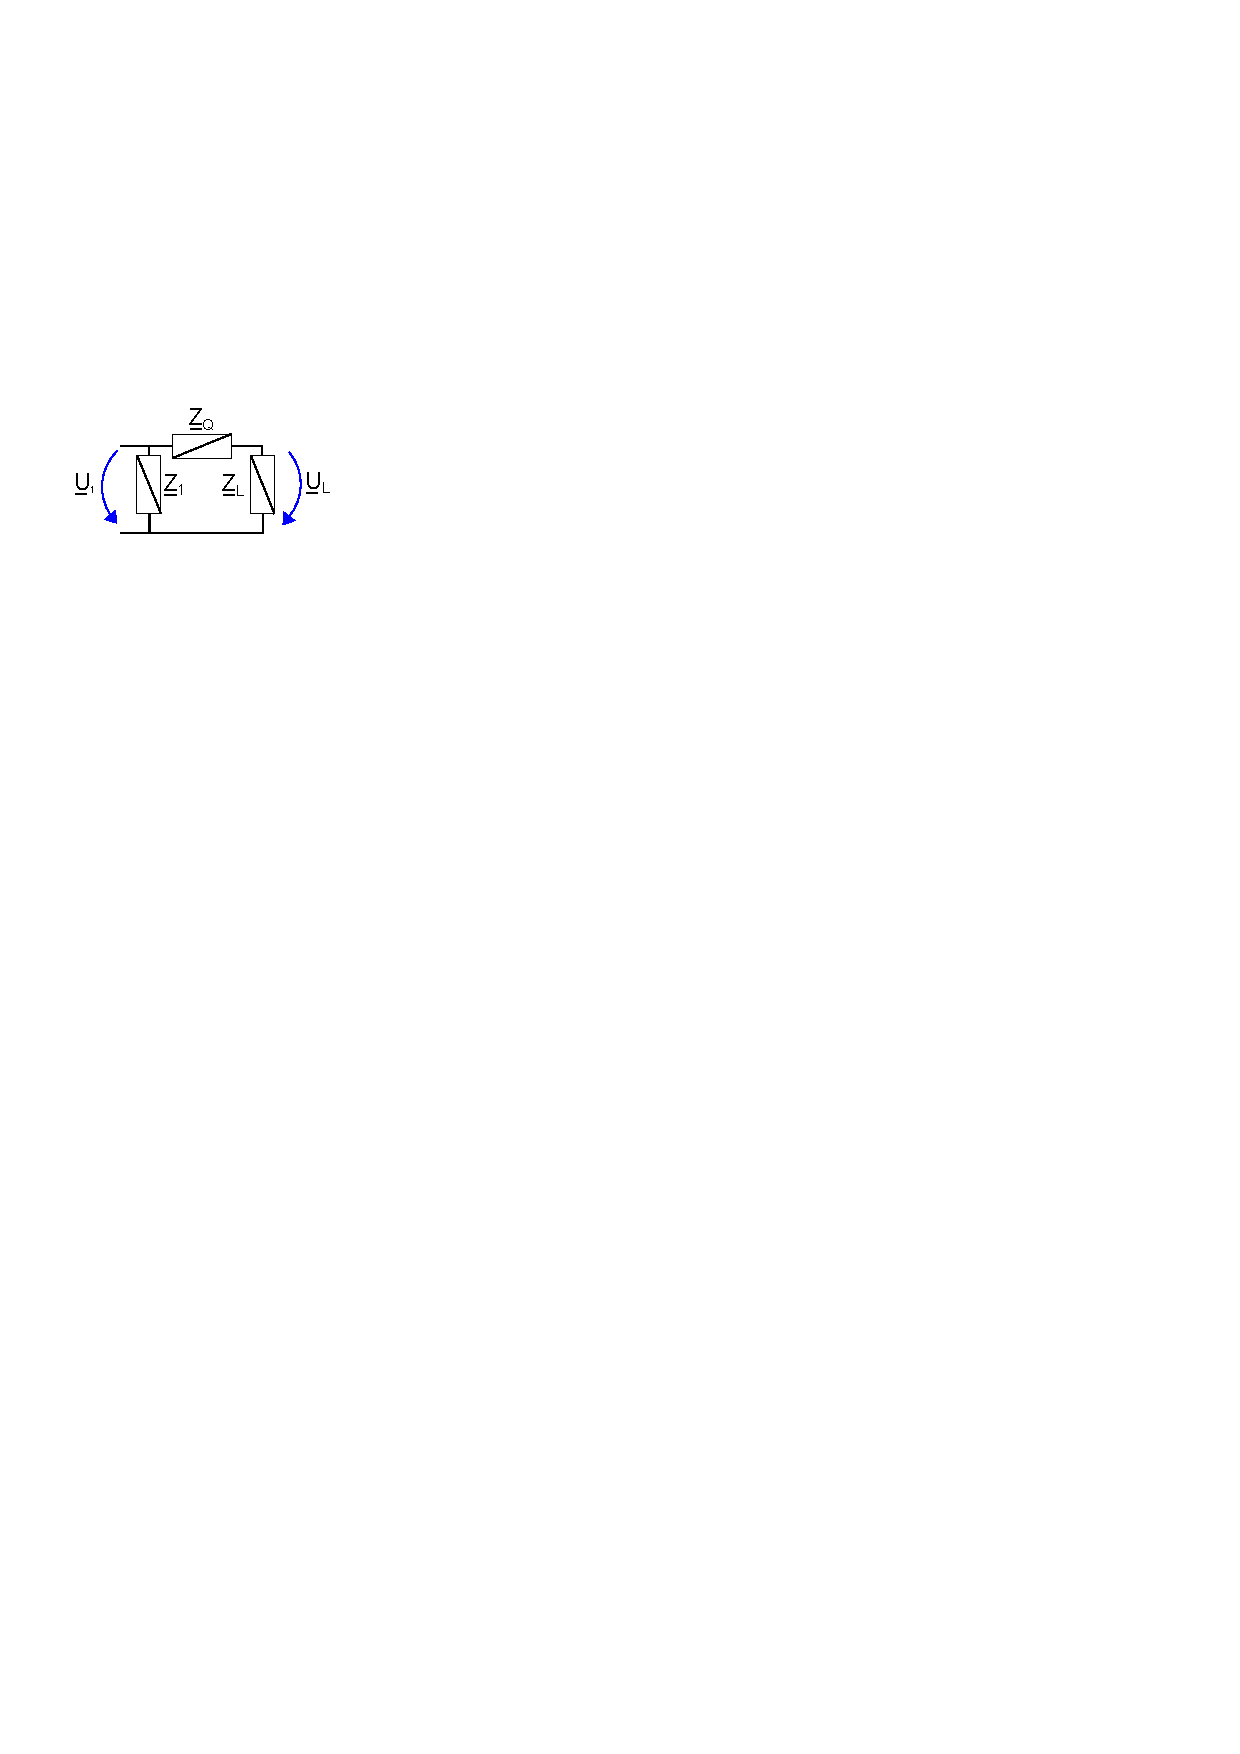
\includegraphics[width=\textwidth]{./images/WechselDrehstromrechnung.pdf}
\end{minipage}
\begin{minipage}[rt]{9cm}
	\begin{equation*}
		\underline{U}_L = \frac{\underline{Z}_L}{\underline{Z}_L + \underline{Z}_Q} \cdot \underline{U}_1
	\end{equation*}
\end{minipage}
  